\pdfminorversion=5
\pdfobjcompresslevel=2

\RequirePackage[l2tabu, orthodox]{nag}

\documentclass[sigplan, screen]{acmart}

\usepackage[T1]{fontenc}
\usepackage[utf8]{inputenc}

\usepackage{microtype}
\usepackage{listings}
\usepackage{color}
\usepackage{xspace}
\usepackage{balance}
\usepackage{todonotes}
\usepackage{subcaption}
\usepackage[all]{nowidow}
\usepackage{tikz}
\usepackage[scaled]{beramono}
\usepackage{booktabs}
%\usepackage[bookmarks=false,colorlinks=true,allcolors=black,breaklinks]{hyperref}
\usepackage{cleveref} % Keep me last so that I can
                      % reset other counters

%\setlength{\belowcaptionskip}{-15pt} % Bear with me

\newtheorem{definition}{Definition}

% Copyright
%\setcopyright{none}
%\setcopyright{acmcopyright}
%\setcopyright{acmlicensed}
%\setcopyright{rightsretained}
%\setcopyright{usgov}
%\setcopyright{usgovmixed}
%\setcopyright{cagov}
%\setcopyright{cagovmixed}

% DOI
%\acmDOI{10.475/123_4}

% ISBN
%\acmISBN{123-4567-24-567/08/06}

%Conference
\acmConference[SLE'18]{International Conference on Software Language Engineering}{November 2018}{Boston, MA, USA}
\acmYear{2018}
\copyrightyear{2018}

\acmPrice{15.00}

%\acmBadgeL[http://ctuning.org/ae/ppopp2016.html]{ae-logo}
%\acmBadgeR[http://ctuning.org/ae/ppopp2016.html]{ae-logo}

\hypersetup{%
	pdftitle={},
	pdfauthor={},
	pdfkeywords={}
}

% Usual suspects
\newcommand*{\ie}{i.e.,\@\xspace}
\newcommand*{\eg}{e.g.,\@\xspace}
\newcommand*{\cf}{cf.\@\xspace}

\makeatletter
\newcommand*{\etc}{%
	\@ifnextchar{.}%
	{etc}%
	{etc.\@\xspace}%
}
\makeatother

\newcommand*{\de}{$\Delta$\@\xspace}
\newcommand*{\ds}{$\Delta$s\@\xspace}
\newcommand*{\db}{$\Delta$-based\@\xspace}
\newcommand*{\M}{\mathcal{M}}

\newcommand*{\diff}{\textit{diff}\@\xspace}
\newcommand*{\patch}{patch\@\xspace}
\newcommand*{\prism}{\textsc{Prism}\@\xspace}

% Listings
\definecolor{keywordscolor}{RGB}{127, 0, 85}
\definecolor{stringcolors}{RGB}{42, 0, 255}
\definecolor{commentscolor}{RGB}{63, 127, 95}
\definecolor{annotationscolor}{RGB}{100, 100, 100}
\definecolor{lstbgcolor}{RGB}{245, 245, 245}

% Custom Java
\lstset{
	language=Java,
	%	mathescape=true,
	literate={->}{$\rightarrow$}{1},
	keywordstyle=\color{keywordscolor}\bfseries,
	commentstyle=\color{commentscolor},
	stringstyle=\color{stringcolors},
	basicstyle=\ttfamily\tiny,
	captionpos=b,
	numbers=left,
	%	backgroundcolor=\color{lstbgcolor},
	%	framexleftmargin=20pt,
	xleftmargin=17pt,
	aboveskip=\bigskipamount,
	belowskip=\bigskipamount,
	%	frame=tb,
	tabsize=2,
	breaklines=true
}

% Rascal
\lstdefinelanguage[]{Rascal}[]{Java}
{
	morecomment=[l]{\@},
	morekeywords={alias, tuple, lrel, data, str, value, int, list}
}

\usetikzlibrary{shapes.callouts, shadows}
\tikzset{author comment/.style={draw, fill=white, thick, drop shadow}}

\newcommand{\Comment}[3]{%
	\ifthenelse{\boolean{CommentON}}{%
		\raisebox{-.5ex}
		{\tikz
			\node[x=1ex, y=1ex, inner sep=.5ex,
			rectangle callout,
			callout pointer width=.7ex,
			callout relative pointer={(1.5,-0)},
			author comment]
			{\footnotesize\textsf{#1}};}~%
		\textsf{[}\,\textcolor{#2}{#3}\,\textsf{]}\xspace
	}{} %else
}

\newcommand{\td}[1]{\Comment{TD}{blue}{#1}}
\newcommand{\fc}[1]{\Comment{FC}{red}{#1}}


\newboolean{CommentON}
\setboolean{CommentON}{true} % to disable the comments set CommentON to false in the main doc

\begin{document}
\title{``\emph{Free the languages!}''}
\titlenote{Seriously:~Towards Shape-diverse DSLs?}
%\title{Towards Shape-diverse languages}
%\titlenote{Models are synchonized, not DSLs, though}
\subtitle{Language Engineering across Technological Boundaries}
%\subtitlenote{The full version of the author's guide is available as
%		\texttt{acmart.pdf} document}

\author{Benoit Combemale}
\authornote{FIXME:~Alphabetical order for now}
\affiliation{
	\institution{Université Toulouse-Jean-Jaurès}
	\city{Toulouse}
	\country{France}
}
\email{benoit.combemale@irit.fr}

\author{Fabien Coulon}
\affiliation{
	\institution{Université Toulouse-Jean-Jaurès \& Obeo}
	\city{Toulouse}
	\country{France}
}
\email{fabien.coulon@irit.fr}

\author{Thomas Degueule}
\affiliation{
	\institution{CWI}
	\city{Amsterdam}
	\country{Netherlands}
}
\email{degueule@cwi.nl}

\author{Tijs van der Storm}
\affiliation{
	\institution{CWI \& U of Groningen}
	\city{Amsterdam}
	\country{Netherlands}
}
\email{storm@cwi.nl}

% The default list of authors is too long for headers.
%\renewcommand{\shortauthors}{B. Trovato et al.}

\begin{abstract}
Domain-Specific Languages (DSLs) manifest themselves in remarkably diverse shapes, ranging from internal DSLs embedded as a mere fluent API within a programming language, to external DSLs with dedicated syntax and tool support.
% engineered using one of many language workbenches.
%
Although different shapes have different pros and cons, combining them for a single language is problematic:~language designers usually commit to a particular shape early in the design process and it is hard to reconsider this choice later on.
%
%Theoretically, this diversity should enable language designers to combine the strengths of multiple language engineering technologies in the development of a single DSL and enable language users to manipulate their abstractions in the most appropriate shape for the task at hand (\eg~domain modeling vs. system integration).
%In practice, however, combining multiple language implementation techniques is problematic.
%Language designers usually commit to a particular technology (\eg~Spoofax, EMF, Racket) and a particular shape (\eg~internal, external, API) early in the design process and this choice can hardly be reconsidered later on.
%
In this \emph{new ideas} paper, we envision a language engineering approach enabling (i) language users to manipulate their abstractions in the most appropriate shape according to the task at hand, and (ii) language designers to combine the strengths of different technologies for a single DSL. 
%support of multiple shapes for a single DSL to better fit the various tasks to be performed with it. \td{Meh}
%report on early experiments and lessons learned building an incremental synchronization mechanism for \emph{metamorphic DSLs}.
%
We report on early experiments and lessons learned building \prism, an incremental technique for synchronizing multiple shapes of a DSL.
We illustrate its applicability in the engineering of a simple shape-diverse DSL implemented in Rascal, EMF, and Java.
%Metamorphic DSLs are languages whose different constituents (syntax, semantics, tools) can be implemented using various language engineering technologies and which can adapt their shape to a particular user or task.
%Taking as an example a simple metamorphic FSM language implemented simultaneously in three technological spaces (Rascal, EMF, a fluent API in Java), we show how the same FSM models can be manipulated indifferently under various shapes (a textual program in Rascal, a graphical projection in EMF, a Java AST).
%This opens up the possibility to, \eg animate an FSM model in EMF while it is executed by an interpreter written in Rascal.
%
We hope that our initial contribution will raise the awareness of the community regarding these notions, and that the challenges we identify encourage future research.
%We intend to raise the awareness of the community on these notions, identify some of the challenges we encountered along the way, and encourage future investigations.
\end{abstract}


%
% The code below should be generated by the tool at
% http://dl.acm.org/ccs.cfm
% Please copy and paste the code instead of the example below.
%
 \begin{CCSXML}
	<ccs2012>
	<concept>
	<concept_id>10011007.10011006.10011050.10011017</concept_id>
	<concept_desc>Software and its engineering~Domain specific languages</concept_desc>
	<concept_significance>500</concept_significance>
	</concept>
	</ccs2012>
\end{CCSXML}

\ccsdesc[500]{Software and its engineering~Domain specific languages}

%\keywords{domain-specific language, metamorphic dsl, language workbenches}

%\begin{teaserfigure}
%	\includegraphics[width=\textwidth]{sampleteaser}
%	\caption{This is a teaser}
%	\label{fig:teaser}
%\end{teaserfigure}

\maketitle

\section{Introduction \& Motivating Example}
One of the first steps in designing a new Domain-Specific Language (DSL) is to choose which \emph{language vehicle} (LV) will be used to engineer it.
We define a LV as the technological means for implementing a language.
This includes language workbenches as well as programming languages and ontology languages, to name a few.
%A language vehicle may pertain to any \emph{technological space} (TS) such as grammarware, modelware, PLware, \etc.
The notion of language vehicle is orthogonal to the distinction between technological spaces (\eg~grammarware, modelware~\cite{kurtev2002technological}); between graphical and textual syntax; between internal, embedded, and external DSLs,~\etc.
%\footnote{In this paper, we build upon \citeauthor{kurtev2002technological}'s view of a TS:~``a working context with a set of associated concepts, body of knowledge, tools, required skills, and possibilities''~\cite{kurtev2002technological}.}
%In addition, we consider a cohesive set of tools in a given TS (\eg~a particular language workbench) as a separate TS.
For instance, we consider Rascal~\cite{klint2010easy} and Spoofax~\cite{kats2010spoofax} as two distinct language vehicles within the broader technological space of grammarware and meta-programming; EMF~\cite{steinberg2008emf} and UML~\cite{fowler2004uml} (using Profiles~\cite{selic2007systematic}) as two distinct language vehicles within the broader technological space of modelware.
LVs usually come with their own meta-languages for expressing the various aspects of a DSL:~abstract syntax, concrete syntax, static and execution semantics, tools, \etc.
%Examples of prominent LV include meta-modeling environments such as EMF~\cite{steinberg2008emf}, meta-programming environments such as Rascal~\cite{klint2010easy} and Spoofax~\cite{kats2010spoofax}, projectional environments such as MPS~\cite{voelter2013language}, plain old programming languages such as Racket~\cite{felleisen2018programmable} or Scala~\cite{hofer2010modular}, and language workbenches (LWBs) in general~\cite{erdweg2015evaluating}.
%\td{Sentence above could be shortened/removed}
As implementation techniques radically differ from one LV to another, this initial design choice commits the development of a DSL in a set direction that can hardly be reconsidered later.

From the language designer's point of view, however, every LV has its own strengths.
The ecosystem around EMF excels in the definition of user-friendly editors and persistence frameworks for large models, while the Rascal environment excels in the definition of interpreters and refactoring tools.
%On the other hand, the flexibility of manipulating the concepts of a DSL through a fluent API, using the capabilities of a general-purpose programming language, is unmatched.
The benefits of various LVs are also visible from the language users' point of view.
While domain experts may prefer to manipulate domain concepts through a dedicated syntax, advanced users (\eg~system integrators) may favor the flexibility of a fluent API in their favorite programming language to manipulate the very same constructs.
%However, it is currently not possible to \emph{combine the strengths of multiple LV to engineer a single DSL}.
%\td{Why?}

Let us consider a simple finite-state machine (FSM) language as a motivating example.
As depicted in \Cref{fig:motivating-fsm}, one would like to combine the strengths of multiple LVs to engineer this DSL.
Rascal could be used to develop its interpreter, a set of refactoring tools (\eg~state collapsing and minimization), and a textual editor; EMF to develop a graphical animator for debugging FSM models and a persistence layer; Java to offer a fluent API for advanced users who focus on its integration with other system concerns.

\begin{figure}[bt]
	\centering
	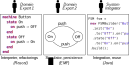
\includegraphics[width=\columnwidth]{figures/motivating-fsm-simplified-2}
	\caption{Three incarnations of the same FSM model in three language vehicles:~different representations and tools for different users and tasks.}
	\label{fig:motivating-fsm}
\end{figure}

Using today's techniques, it is possible to define the same FSM language in these three LVs separately.
It is not possible, however, to apply the tools of a given LV on the models or programs created in another LV---for instance, animating a FSM model written in EMF using the Rascal interpreter, or synchronizing a textual FSM model in Rascal with its equivalent incarnation as a Java AST.
Achieving this goal requires to \emph{efficiently synchronize the diverse representations of the same model in different LVs}; for instance to let the FSM interpreter written in Rascal update its own representation of an FSM model after each execution step and synchronize it with the representation of the same model in EMF for animation purposes.

In this paper, we envision a language engineering approach enabling (i) language designers to combine tools from multiple LVs to engineer diverse shapes for a single DSL and (ii) language users to manipulate language constructs in the most appropriate shape.
%We endeavor to show \emph{how to break down the barriers between different vehicles so that language designers can combine the strengths of each in the engineering of a single DSL, and language users can synchronize their models across various shapes}.
%\emph{Metamorphic synchronization} refers to the possibility of synchronizing different incarnations of the same model in different shapes of a language, \ie~in different vehicles.
%As different vehicles rely on radically different theories, a successful approach for bridging them must thus \emph{align} \td{!no!} them in some way.
We present the notion of shape-diverse DSL in greater depth in \Cref{sec:shapes}.
We then present our prototype approach, \prism, in \Cref{sec:prism}, and discuss our implementation of a shape-diverse FSM language in \Cref{sec:eval}.
Finally, we discuss open questions and next steps in \Cref{sec:discussion}.

\section{Synchronizing Incarnations with \prism}
\label{sec:prism}

\Cref{fig:prism} depicts our prototype approach to the problem of synchronizing various incarnations of a model, \prism.
Our approach keeps the LVs fully independent and uses \prism as a communication bus between them.
The key idea is that every change occuring on one incarnation is shipped to all other incarnations of the same model in the form of a \emph{patch}.
An alternative approach is Change Propagation of View Models
by Logic Synthesis using SAT solvers~\cite{DBLP:conf/etaps/SemerathDHV16}, which propagate changes from models to views using traceability links. This is in contrast with our approach where the underlying model is not materialized.
This patch represents the exact set of changes that occured on one incarnation.
It allows to synchronize incarnations online efficiently without requiring serialization or a full traversal of any of the incarnation.
\prism keeps track of a matrix that associates every conceptual model to its incarnations in various LVs.
When a change occurs on one incarnation, for instance resulting from a user edit or an execution step of an interpreter, the LV hosting this incarnation generates a patch describing the change as a set of CRUD-like operations.
In our prototype implementation, the structure of this patch is prescribed by the Rascal ADT shown in \Cref{lst:delta-adt}, largely inspired by the \emph{edit scripts} used by \citeauthor{rozen2017towards}~\cite{rozen2017towards}.
Essentially, patches consist of a set of operations attached to identities~\cite{klint2016model} that represent particular objects in the model.
To ensure that every LV can apply the operations on the right elements, identities are preserved across LVs and, in our case, they are represented by URIs~\cite{berners2004uniform}.

%On the edition of an incarnation of a model, its containing LV creates a patch describing the changes. The LV ships the patch to \prism, which then propagates the patch to every other incarnation of the same model. \prism use a simple matrix that keeps track of the associations between models and their incarnations in various LVs.
%Every LV is then responsible for updating its own incarnation by interpreting the patch.

\begin{figure}[bt]
	\centering
	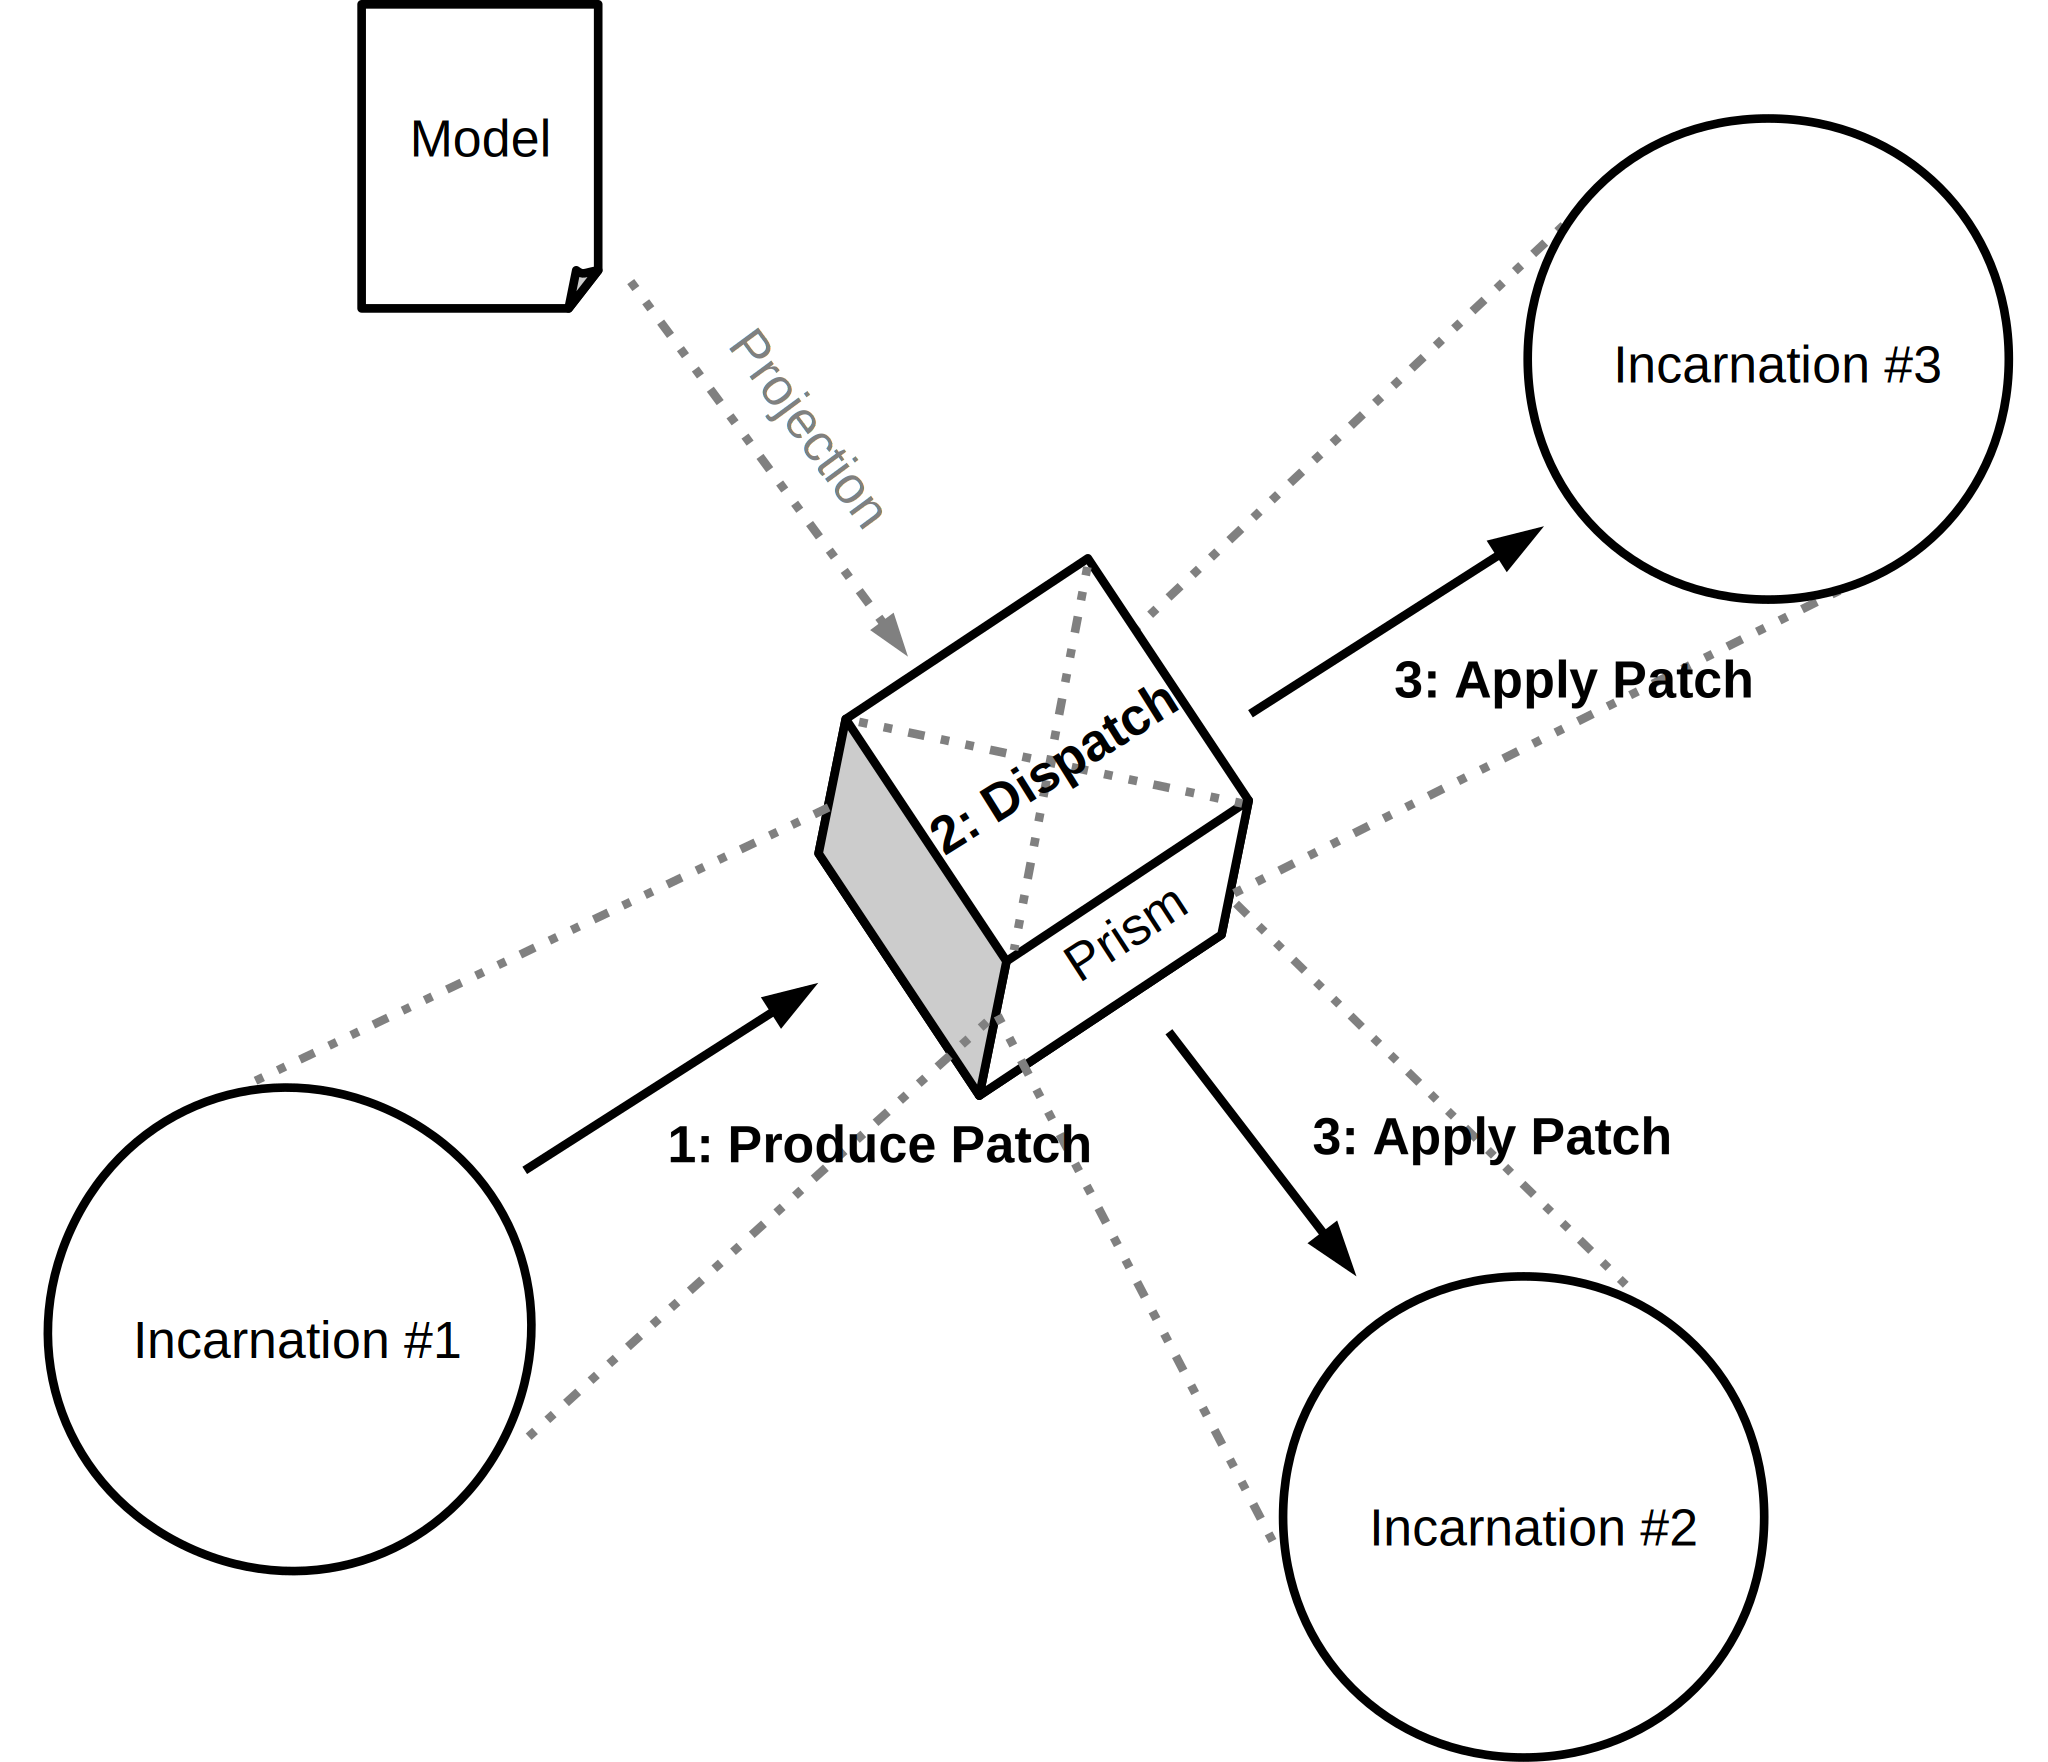
\includegraphics[width=.6\columnwidth]{figures/prism}
	\caption{Using \prism to synchronize three incarnations of the same model. Here, a change occurs on Incarnation \#1 and the resulting patch is shipped to Incarnation \#2 and \#3.}
	\label{fig:prism}
\end{figure}


%Representations of the same model in various LVs are kept in memory to enable online synchronization of the same models manipulated by different stakeholders in different shapes.
%When a changes occurs on either incarnation, the hosting LV is responsible for generating the corresponding \emph{patch}.
%The communication bus then ships this patch to all the other LVs that hold an alternative incarnation of this model.
% (aka. \de or edit script~\cite{rozen2017towards}), that stores the changes on the model that have been realized on this LV.

Every LV then interprets the patch in its own way to keep the representation synchronized.
In EMF, for instance, the patch is interpreted as a set of changes that impact a model conforming to an Ecore metamodel, while in Rascal it is interpreted as a set of changes that impact an ADT value.

As mentioned earlier, each LV may want to preserve extra shape-specific information across the patches.
A textual editor in Rascal, for instance, needs to keep some of the parsing information to maintain layout whenever patches are applied.
So it should be possible to apply the patch while maintaining the extra information specific to a given LV.
Intuitively, our approach supposes that all the information that does not directly relate to the constructs of a language is ``extra'' and therefore should not be part of the patch itself.
There might be cases where sharing extra-information from one shape to the other is desirable, for instance to share layout information between two textual editors.
We discuss this point further in \Cref{sec:discussion}.
%Automatically generating language implementations in different LV is beyond the scope of this paper.
%Instead, given various shapes of a language, implemented by hand, we provide the means to automatically synchronize the projections of a model.

New LVs can be connected to \prism by implementing a simple interface that consists of two operations, namely (i) \emph{produce} which creates a patch materializing the changes on an incarnation and notifies \prism, and (ii) \emph{apply} which receives a patch from \prism and interprets it to update an incarnation, taking into account the specificities of the LV.
The way changes are detected in an incarnation and patches are produced is not prescribed by our approach.
For instance, our Rascal implementation computes patches from a \emph{diff} operation between two ADT values, while our EMF implementation captures the result of transactions on an Ecore model to produce the patches.
The produce and apply operations are implemented once for every LV and do not have to be re-implemented for every language.
%Connecting a LV to \prism consist of producing and interpreting patches for a language.
%A LV has the task of watching changes happening on a incarnation of a model conform to a targeted language and notifying \prism.
%The LV describes the changes in a patch. The patch is an edit script where each operation follows the CRUD-like patch definition.
%After the production of the patch the LV has to notify the \prism.
%In the opposite way a LV can be notified by a patch from the \prism that a change occurred in the model.
%The LV has to interpret this notifying patch to update its own incarnation of the model.
%The interpretation follows the edit script and for each operation applies a change on the incarnation of the model.

A cornerstone artifact in \prism is the dispatch mechanism that routes patches to the appropriate incarnations.
%\prism connects LVs and provides a dispatch mechanism to exchange patches between incarnations of a same model.
When receiving a patch, \prism looks up its internal matrix to determine which other incarnations of the same model should be updated.
%at the corresponding model to find other incarnations of the same model.
The patch is then copied and routed accordingly.
%The lookup is implemented by a matrix internal to \prism linking models to their incarnations. This matrix is kept updated by connected LVs declaring which incarnations of which model they manage.
%\prism addresses the synchronization of different incarnations of same models that is a complementary problem of the collaborative edition.
Our current implementation of the dispatch mechanism is kept simple, and we leave for future work the support of concurrent edits on different incarnations of the same model. This would scale \prism to advanced scenarios that go beyond the scope of this paper, such as collaborative editing.
%Our approach only deals with sequential edition of incarnations and thus complementary work on concurrency in our dispatch mechanism could allow collaborative edition scenarios.

%\td{Highlight incrementality, \ie~we're not Xtext, $\neq$ full de-/re-serialization}

\begin{lstlisting}[label=lst:delta-adt, caption={CRUD-like patch definition in Rascal.}, language=Rascal, float=tb]
@doc{A patch consists of a sequence of edits}
alias Patch = tuple[Id root, Edits edits];

@doc{Edits are operations attached to object identities}
alias Edits = lrel[Id obj, Edit edit];

data Edit
  = put(str field, value val)
  | unset(str field)
  | ins(str field, int pos, value val)
  | del(str field, int pos)
  | create(str class) 
  | destroy();
\end{lstlisting}

\section{A Shape-Diverse FSM Language}
\label{sec:eval}

To illustrate \prism, we build a shape-diverse FSM language conjointly in Rascal, EMF, and Java.
\Cref{fig:3fsms} depicts the implementation of the abstract syntax of this FSM language in the three LVs.\footnote{The implementation of \prism and the FSM example are available on a companion webpage:~\url{https://github.com/fcoulon/prism/}}
The corresponding incarnations are those given in \Cref{fig:motivating-fsm}.

\begin{figure}[bt]
	\centering
	\begin{subfigure}[t]{.3\columnwidth}
		\vskip 0pt
		\begin{lstlisting}[label=lst:fsm-adt, language=Rascal, numbers=none, xleftmargin=0pt, tabsize=1, aboveskip=0pt, belowskip=0pt, abovecaptionskip=0pt, showlines=true]


data Machine(Id uid) =
	Machine(str name,
		list[State] states,
		Ref[State] initial);

data State(Id uid) =
	State(str name,
		list[Trans] trans);

data Trans(Id uid) =
	Trans(str event,
		Ref[State] target);


		\end{lstlisting}
		\caption{Rascal ADT}
	\end{subfigure}
	\vrule
	\enskip
	\begin{subfigure}[t]{.26\columnwidth}
		\vskip 5pt
		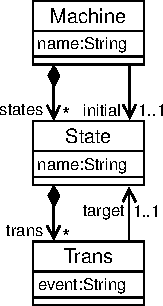
\includegraphics[width=\textwidth]{figures/fsm-mm}
		\vskip 4pt
		\caption{Ecore MM}
	\end{subfigure}
	\enskip
	\vrule
	\enskip
	\begin{subfigure}[t]{.35\columnwidth}
		\vskip 0pt
		\begin{lstlisting}[label=lst:fsm-api, language=Java, numbers=none, xleftmargin=0pt, tabsize=1, aboveskip=0pt, belowskip=0pt, abovecaptionskip=0pt]
class Fsm {
	Fsm(String name);
	State init(String name);
	State state(String name);
	Fsm end();
}
class State {
	State state(String name);
	Trans tgt(String name);
	Fsm end();
}
class Trans {
	Trans tgt(String name);
	State on(String event);
	Fsm end();
}
		\end{lstlisting}
		\caption{Java API}
	\end{subfigure}
	\caption{Three shapes of an FSM language; the corresponding incarnations are those depicted in \Cref{fig:motivating-fsm}.}
	\label{fig:3fsms}
\end{figure}

We use Rascal to define a textual editor and a simple transformation that inserts a new state in a machine.
We use EMF to define two graphical editors:~a classical tree editor and a domain-specific representation with Sirius.
We build the Java API following a simple systematic convention, so as to easily pinpoint which parts of the Java AST have changed (to compute a patch) or need to be updated (to apply a patch).

We use \prism to bridge these shapes.
%\prism is used to bridge these different shapes.
Whenever an incarnation of the FSM model is updated, the LV in which the change happens produces a patch (\cf\Cref{lst:delta-adt}) that is shipped to the other LVs through the dispatch mechanism of \prism.
Every LV interprets the patch in its own way to keep its incarnation updated, accounting for the extra information it has to manage (\eg~layouts within the textual and graphical editors).
A simple matrix, internal to \prism, keeps track of which model each incarnation is projecting to route the patch to the right incarnation.

%Rascal is providing a textual editor, Ecore provides a graphical editor and we used the Java editor for the fluent API.
%In our manipulation we were able to edit an incarnation of a model in one editor and see the change applied in others editors.
%By using an editor, we were able to benefit of the result of the tooling in others incarnations, i.e., using the content assist of Java is also updating other editors.
%We also observe some de-synchronization happening due to the partially unaligned FSM implementation in Java.

While the Rascal and EMF shapes synchronize seamlessly, we noticed a number of challenges with the Java API.
As the Java API inherits the (domain-agnostic) tooling of Java itself, it lacks the domain knowledge necessary to always generate correct patches.
Due to the lack of domain-specific static semantics, a well-formed Java program may indeed produce an ill-formed FSM that cannot be interpreted by the other shapes.
Besides, our prototype implementation does not account for complex string manipulation when invoking the API or use of variables.
However, we believe that these are purely engineering concerns and that enough effort spent on the Java API shape would provide a flawless experience.

%The Java fluent API shape tends to break more easily the synchronization of their incarnations of models than the other shapes.
%Indeed this shape of FSM language is an embedded language and has to rely on the host language for both the tooling and the expressiveness.
%In the case of Java as host language, the validation service provided by the editor has no knowledge about the FSM language.
%It makes harder for the user to detect mistakes such as typo. The FSM model can be in unnoticed dirty state and this can lead to the production of dirty Patches.
%In the opposite the incarnation of the model can receive inapplicable Patches in this technological space.

%Another example in the Java TS of problem encountered is the constraints from the host language.
%We choose to represent a State by the method state() or by the method initial().
%As the initial State is unique, we enforce its declaration as the first method invocation in the FSM.
%This solution solve the uniqueness but enforce the first state to be initial.
%Thus with this representation of FSM, receiving a Patch telling to reference the second state of an FSM as the initial state is not possible due to the expressiveness of the API and this result in the desynchronization of the incarnation of the model.
%
%The inconsistency of the incarnations of a model happen when one of them produce a dirty Patch or when one of them can't apply a Patch.

\section{Open Questions \& Next Steps}
\label{sec:discussion}
From the language designers and users points of view, the rigidity of SLE must be fought.
In this paper, we have stressed the importance of shape-diverse DSLs and have proposed a first prototype approach, \prism, towards this vision.
Below, we list some open questions that arose during our experiments, as well as a list of research problems to address in the future.

\paragraph{Open-world vs. Closed-world}
Implementers of a synchronization mechanism for shape-diverse DSLs may opt for the closed-world or open-world assumption.
In the former, one assumes that all LVs are known beforehand, while in the latter new LVs may be connected at any point in time, for instance using our \emph{produce/apply} interface for patches.
Although the closed-world assumption eases the definition of a common patch formalism on which all LVs agree, it hampers evolution and adaptability.

\paragraph{Patch formalism}
We opted for patches in the form of edit scripts~\cite{rozen2017towards}.
We do not really know if our patch formalism is sufficient:~what if you want to connect another formalism; is there anything missing?
We don’t care how patches are obtained. Diff is \emph{a} way to get there (as in the Rascal implementation), but obtaining the list of changes through other means (e.g., a transaction on a tree editor in EMF) is just as valid.
It should be possible to generate shapes from a common language definition, or generate a shape from another one (\eg~grammar to API generation~\cite{IThinkGPCEHadAPaperOnThat}).

\paragraph{Automatic shape generation}
It may or may not be possible to automatically generate a shape from another.
In our prototype implementation, we are able to Ecore $\leftrightarrow$ Rascal.

\paragraph{Towards collaborative modeling}
A smarter dispatch mechanism would enable collaborative editing, distributed synchronization, \etc;
We need a mechanism to valid produced Patches and their interpretations to detect desynchronization of incarnations (what should we do then? roll back? fix Patch?)

\paragraph{Challenges of internal DSLs}
Transforming context-heavy Java ASTs is challenging; our tool is stupid in that respect; DIY.

\paragraph{Towards metamorphic DSLs}
We view this initial contribution as a first step towards \emph{metamorphic DSLs}~\cite{acher2014metamorphic}.

\paragraph{LSP \& Monto}


\paragraph{Others}
Our approach goes beyond what is described here. \eg synchronizing an outline view, a debugger, live modeling, w/e; also, we are AS-centric, but one could imagine something radically different;
Delta/edit scripts are known (ref?), ``pivot'' formalisms are---infamously---known, we combine both in a new context; why? what do we get from that?


\clearpage
\balance
\bibliographystyle{ACM-Reference-Format}
\bibliography{main}

\end{document}
